\documentclass{paper}
\usepackage[utf8]{inputenc}

\title{wsp}
\author{wsp }
\date{November 2019}

\usepackage{natbib}
\usepackage{graphicx}

\begin{document}



\section{Introdução}
O curso é ministrado por Carlos Ferraz (CC) e Eduardo Tavares (EC). Tem como objetivo  fazer com que os alunos entendam o funcionamento dos sistemas de software que fornecem uma infra-estrutura através da qual aplicativos (browsers Web, editores de texto, planilhas eletrônicas, jogos, etc.) podem interagir com o hardware. Ao final da disciplina, os alunos devem apresentar uma compreensão dos principais mecanismos necessários para se construir tal infra-estrutura, considerando os dois papéis que ela desempenha: de mecanismo de abstração para a plataforma de hardware subjacente e de gerenciador de recursos diversos como memória, capacidade de processamento e dispositivos de armazenamento e de entrada e saída. Nesta disciplina, o software de infra-estrutura está dividido em duas partes:  o sistema operacional; e o  middleware. Essa disciplina funciona em harmonia com as outras duas disciplinas de infra-estrutura, a de hardware e a de comunicação, e juntas as três fornecem um panorama razoavelmente completo sobre o funcionamento de um sistema computacional.
\citep{chamada1}
\citep{chamada2}
\citep{chamada3}
\citep{chamada4}
\begin{figure}[h!]
\centering
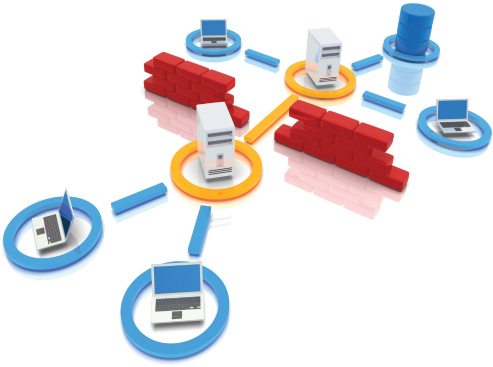
\includegraphics[scale=0.6]{infraSoftware.jpg}
\caption{Infraestrutura de Software}
\label{fig:Infraestrutura de Software}
\end{figure}

\section{Relevância}
A utilização de sistemas distribuidos é muito comum no mundo coorporativo,devido a isso  um bom profissional na área de computação deve ssaber exatamente como eles funcionam e se comunicam,o curso de infraestrutura de software proporcionará essas habilidades aos seus alunos. Além disso, o aluno irá aprender novas formas de programação.
\section{Relação com outras cadeiras}
IF669- INTRODUCAO A PROGRAMACÃO 
O aluno precisa dominar os conhecimentos básicos da programação,para assim cursar a cadeira de infra de software,já que eles servirão de base para os conteúdos aprensentados na disciplina.
\bibliographystyle{plain}
\bibliography{wsp}
\end{document}